\chapter{Background}

In this chapter we introduce some general notions as well as a more deep understanding of what P systems and Petri nets are.

\section{Basic Definitions}

\begin{definition}[Multiset]
Let $U$ be an arbitrary set. A multiset over U is a mapping \newline $m : U \rightarrow N$.
The multiplicity of an element $u$ in $m$ is given by the natural number $m(u)$.
Given the multisets $m$ and $m'$, we write $m \subseteq m'$ if $m(u) \leq m'(s)$ for all $u \in U$, 
while $\oplus$ denotes their multiset union: $m \oplus m' = m(u) + m'(u)$ for each $u$.

\end{definition}


\begin{definition}[Alphabet]
An alphabet is a finite nonempty set of abstract symbols. Given an alphabet $V$, we denote by $V^*$
the sets of all finite strings of elements in $V$, including the empty string $\lambda$.
Every string $v \in V$ describes a multiset over $V$.
\end{definition}

\section{P Systems}

Membrane computing is a branch of natural computing, introduced by Gheorghe Paun with the definition of P systems in \cite{puaun2000computing,puaun2002membrane,paun1999computing}.

Membrane systems are based upon the notion of \textit{membrane structure}, which is a structure composed by several cell-membranes, hierarchically embedded in a main membrane called the \textit{skin membrane}.
The membranes delimit \textit{regions} and we associate with each region a set of \textit{objects}, described by some symbols over an alphabet, and a set of \textit{evolution rules}.
In the basic variant, the objects evolve according to the evolution rules, which can modify the objects to obtain new objects.
The evolution rules are applied in a \textit{maximally parallel manner}: at each step, all the objects which can evolve should evolve.
If a computation \textit{halts}, so no further evolution rule can be applied, the result of the computation is defined to be the number of objects in a specified membrane.

\begin{definition}[P system]
A P system (of degree $d$, with $d \geq 1$) is a tuple
\[ \Pi = (V,\mu,w^0_1,...,w^0_d,R_1,...,R_d, i_0)\]
where:
\begin{enumerate}
  \item $V$ is an alphabet; its elements are called objects;
  \item $\mu$ is a membrane structure consisting of $d$ membranes (labeled with $1,2,...,d$);
  \item $w^0_1, 1 \leq i \leq d$, are strings from $V^*$ representing multisets over $V$ associated
  with the regions $1,2,...,d$ of $\mu$;
  \item $R_i, 1 \leq i \leq d$, are finite sets of evolution rules $r$ over $V$, associated 
  with the regions $1,2,...,d$ of $\mu$; these evolution rules are of the form 
  \[ lhs^r \rightarrow rhs^r \]
  where $lhs^r$ is the left hand side of $r$, $rhs^r$ the right hand side of $r$, and both are non-empty multisets over $V$.
  \item $i_0$ is a number between 1 and $d$ which specifies the output membrane of %\Pi;
\end{enumerate}
A P system $\Pi$ as above \textit{evolves} from configuration to configuration as a consequence of the application of (multisets of) evolution rules in each membrane.
Formally, a \textit{configuration} is a tuple $C=(w_1,...,w_d)$, where each $w_i$ is a multiset of objects (with $1 \leq i \leq d$).
$C_0=(w^0_1,...,w^0_d)$ is the initial configuration.
\end{definition}

According to \cite{agrigoroaiei2010flattening}, any P system can be flattened to a system of degree 1; we call this type of P systems \textit{flat P systems}.
For the sake of simplicity, from now on when we talk about P systems we are referring to flat P systems.

\begin{definition}[Flat P system]
A flat P system is a P system of degree one
\[ \Pi = (V,\mu,w^0,R) \]

A configuration of $\Pi$ is now a singleton $C=(w)=w$, where $w$ is a multiset of objects over $V$, and 
$C_0=(w^0)=w^0$ is the initial configuration.
\end{definition}

Given two configurations $C=(w)$ and $C'=(w')$, $C$ can evolve into $C'$ if there exists a multiset of evolution rules $\mathcal{R}$ such that the following hold:

\begin{enumerate}
    \item $lhs_\mathcal{R} \leq w$;
    \item there is no rule $r$ in $\mathcal{R}$ such that $lhs^r+lhs_\mathcal{R} \leq w$;
    \item for each object $a \in V$,
    \[ w'(a)=w(a)-lhs_\mathcal{R}(a)+rhs_\mathcal{R}(a)\]
\end{enumerate}

The maximal parallelism is captured by 2. according to which no additional evolution rule can be applied.
3. describe the effect of the application of the rules in $\mathcal{R}$.
To be applied in an evolution step a rule $r$ has to be \textit{enabled}; for a rule $r$ to be enabled in $C=(w)$ means that $lhs(r) \leq w$.
By $C \xRightarrow{\mathcal{R}} C'$ we denote that $C$ evolves into $C'$ due to the application of $\mathcal{R}$.
A finite \textit{computation} of $\Pi$ is now a (finite) sequence of evolutions starting from the initial configuration $C_0$.\newline

The following example will clarify what a P system is and how it evolves.
\begin{example}
\label{ex:flat_membrane}
Consider the following P system:
\begin{description}
   \item $\Pi=(V,\mu,w^0,R)$,
   \item $V=\{a,b,c\}$,
   \item $\mu=[_{1}]_{1}$,
   \item $C_0=w^0=a^2b$,
   \item $R=\{r_1:a \rightarrow b, r_2:a \rightarrow c\}$
\end{description}    
\end{example}

The system is represented in Fig 2.1.

\begin{figure}[h]
\centering

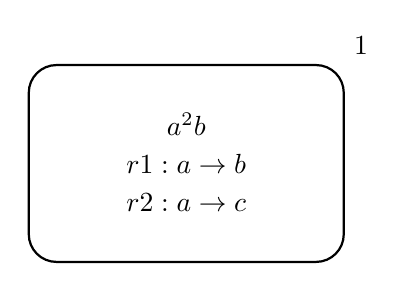
\begin{tikzpicture}
    \draw[thick, rounded corners=10pt] (0, 0) rectangle (4, 2.5) node[above right] {1};
    
    \node at (2, 1.75) {$a^2b$};
    \node at (2,1.25) (rule) {$r1: a \rightarrow b$};
    \node at (2,0.75) (rule) {$r2: a \rightarrow c$};
\end{tikzpicture}

\caption{}
\label{}
\end{figure}

The possibilities to evolve in one step from the initial configuration are: 
\begin{description}
    \item $a^2b \xRightarrow{\mathcal{R}} b^3$ where $\mathcal{R}=r_1^2$,
    \item $a^2b \xRightarrow{\mathcal{R}} bc^2$ where $\mathcal{R}=r_2^2$,
    \item $a^2b \xRightarrow{\mathcal{R}} b^2c$ where $\mathcal{R}=r_1 r_2$
\end{description}

Note that the evolution of $C_0$ is non-deterministic in the sense that there may be different multisets of rules applicable to $C_0$ as described in the example above.

\subsection{Synchronized P systems}

In this section we introduce a new class of P systems, P systems with \textit{synchronization among the rules of the same membrane}.
In the previous section we've seen a kind of synchronization where all regions use their rules in parallel in the maximal mode.
That synchronization that we're interested in is different, more exactly, a rule synchronizing with a non-empty set of rules is applicable at least once only if each rule from the set of rules is applicable at least once.

We call P systems with this kind of synchronization \textit{synchronized P systems}.
They are introduced and studied in \cite{aman2019synchronization,aman2022power}.

\begin{definition}[Synchronized P system]
A synchronized P system is a tuple

\[ \Pi = (V,\mu,w^0,R,\rho) \]

where:
\begin{enumerate}
    \item $(V,\mu,w^0,r)$ is a flat P system;    
    \item $\rho$ is a partial relation defined over the set $R$ of rules specifying
    the synchronization relation over the rules;
    $\rho$ is irreflexive, asymmetric and transitive;
\end{enumerate}
\end{definition}

Let's try to understand better what synchronization means.
Synchronization means to create a relationship between evolution rules, and the rules that are in relation with each other needs to be applied at least one time each in a single evolution step;
if that is not possible then none of this rules can be applied.
So for each rule to be applied in $C$ at least once, each rule has to be enabled in $C$.
We refer to such a relationship between rules with new evolution rules called \textit{synchronization rules}.
A synchronization rule is the composition of rules that are in relationship with each other.
We say that \textit{a synchronization is enabled in $C$} if the corresponding synchronization rule is enabled in $C$. 
So a rule $r$ that compose a synchronization rule $r_s$ can be applied in $C$ only if $r_s$ is applied in $C$ at the same evolution step. 

\begin{definition}[Synchronization rule]
\label{def:sync_rule}
A synchronization rule $r_s$ is a special evolution rule that is the result of the composition of several distinct evolution rules.
Synchronization rules are defined from the partial relation $\rho$ in the following way:\newline
given a set of rules $r_1,...,r_n$ that are in a relationship according to $\rho$, there exists
a synchronization rule $r_s$ of the form:
\[ lhs^{r_1} + \cdots + lhs^{r_n} \rightarrow rhs^{r_1} + \cdots + rhs^{r_n} \] 
such as $\gamma(r_s)=\{r_1,...,r_n\}$ is the set of rules that compose $r_s$.

We use the following notations when we refer to synchronization rules: \newline
given $\gamma(r_s)=\{r_1,...,r_n\}$, $r_s=r_1 \cdots r_n = r_1 \otimes \cdots \otimes r_n$.
\end{definition}

Let's see how the maximal parallelism behaviour is modified when synchronization of rules is used.
\begin{example}
    We modify \hyperref[ex:flat_membrane]{Example 1} adding the synchronization 
    $r_{12} = r_1 \otimes r_2$.\\
    Now there is only one possible way to evolve in one step from the initial configuration:\\
    $a^2b \xRightarrow{\mathcal{R}} b^2c$, where $\mathcal{R}=r_{12}$.
\end{example}

\section{Petri Net}

Here we define in a formal way what a Petri Net is.

\subsection{Petri Nets with Inhibitor Arcs}

Here we extend the latter definition of a Petri Net with the concept of inhibitor arcs.
